%!TeX spellcheck = en-GB
\documentclass[landscape,20pt]{transparents2e}

\usepackage{concrete}
\usepackage{conf}
\usepackage[latin1]{inputenc}
\usepackage[T1]{fontenc}
\usepackage{galois}
\usepackage{url}
\usepackage{theorem}
\usepackage{float}
\usepackage{oldgerm}
\usepackage{xspace}
\usepackage{epic}
\usepackage{ae}
\usepackage{eepic}
\usepackage{ulem}

\usepackage{myfigures}
\usepackage{titlesec}
\usepackage{rotating}
\usepackage{epsfig}
\usepackage[dvipsnames]{color}
\usepackage{NamedColors}
\usepackage[psamsfonts]{amsfonts}
\usepackage{amsfonts,amssymb,amsmath,stmaryrd}
%\usepackage{ecltree}
\usepackage{array}
\usepackage[color,matrix,curve,graph,frame,all]{xy}
\usepackage{fancybox}
\usepackage{picinpar}
\usepackage{pdfpages}
\usepackage{stmaryrd}
\usepackage{lscape,graphicx}
\usepackage{amsmath,amscd}
\usepackage{multirow}
\usepackage{boolean}
\usepackage{selection}
%\usepackage{ulem}
\usepackage{concrete}
\newcommand{\rgives}{$\longleftrightarrow$}
\newcommand{\gives}{$\longrightarrow$}
\newcommand{\conc}[1]{\text{$\left[#1\right]$}}
\newcommand{\myfbox}[1]{\scalebox{0.7}{\fbox{#1}}}
\newcommand{\ldot}{\text{.}}
\definecolor{green1}{rgb}{0,0.4,0}
\definecolor{red2}{rgb}{0.75,0.1,0.1}
\definecolor{blue1}{rgb}{0,0,0.5}
\definecolor{purple}{rgb}{0.5,0.1,0.5}
\definecolor{grey}{rgb}{0.5,0.5,0.5}
\definecolor{white}{rgb}{1,1,1}
\newcommand{\white}{\textcolor{white}}
\newcommand{\grey}{\textcolor{grey}}
\newcommand{\red}{\textcolor{red}}
\newcommand{\blue}{\textcolor{BlueViolet}}
\newcommand{\black}{\textcolor{Black}}
\newcommand{\green}{\textcolor{green1}}
\newcommand{\keep}[2]{#1{#2}{}}
%\newcommand{-}{-}
\newcommand{\fun}{\textcolor{purple}}

\normalem


\newcommand{\myfrac}[2]{\frac{\strut \displaystyle #1}{\strut \displaystyle #2}}
\renewcommand{\frametitle}[1]{\red{\HUGE #1 }}
\newcommand{\articles}[1]{\green{#1}}

\newcommand{\coloredpart}[5]{\ifthenelse{\value{#2}=#3}{#1{#4}#5}{#4}}%
\newcommand{\redpart}{\coloredpart{\red}}
\newcommand{\comment}[1]{}

\newcommand{\displayplan}[2]{\begin{slide}{\frametitle{On the menu today}}

\huge

\vfill

{#1}
\setcounter{mainpart}{0}\begin{enumerate}
\item \addtocounter{mainpart}{1}\redpart{superpartie}{\value{mainpart}}{Rule-based modelling}{}%
\item \addtocounter{mainpart}{1}\redpart{superpartie}{\value{mainpart}}{Kappa}{}%
\item \addtocounter{mainpart}{1}\redpart{superpartie}{\value{mainpart}}{Unbounded bio-molecular compounds}{}%
\item \addtocounter{mainpart}{1}\redpart{superpartie}{\value{mainpart}}{The graph of the sites}{}
\item \addtocounter{mainpart}{1}\redpart{superpartie}{\value{mainpart}}{The graph of the edges}{}%
\item \addtocounter{mainpart}{1}\redpart{superpartie}{\value{mainpart}}{Refinement}{}%
\item \addtocounter{mainpart}{1}\redpart{superpartie}{\value{mainpart}}{Conclusion}{}%
\end{enumerate}
{#2}

\vfill

\end{slide}}


\newcounter{superpartie}
\setcounter{superpartie}{0}
\newcommand{\superplan}{\displayplan{\addtocounter{superpartie}{1}}{}}

\begin{document}

\begin{slide}{}
\thispagestyle{empty}
\newcommand{\Hrule}{\rule{\linewidth}{1mm}}

\vspace*{-2.1cm}

\begin{center}
{\bf \Huge{\confname}} \bigskip\\
\end{center}

\vspace*{0.2cm}

\begin{center}
{\bf{\red{\HUGE{Proving the absence of unbounded polymers
in rule-based models}}}} \bigskip\\
\end{center}

\vspace*{0.2cm}

\begin{center}
{\blue {{\Huge \bf Jerome Feret}}}  \smallskip\\
\huge{DI - \'ENS \bigskip}
%\huge{\lang{\'Equipe Antique}{Team Antique}} \bigskip\\
\end{center}

\vspace*{0.2cm}

\begin{center}
\begin{minipage}{\linewidth}
\hfill\hfill
\begin{minipage}{0.08\linewidth}

\includegraphics[height=1.5cm]{inr_logo_cherch_UK_coul.png}
\end{minipage}\hfill
\begin{minipage}{0.08\linewidth}
  
\includegraphics[height=2.92cm]{ENS_Logo.png}
\end{minipage}\hfill
\begin{minipage}{0.08\linewidth}

\includegraphics[height=2.5cm]{CNRSfilaire-grand.jpg}
\end{minipage}\hfill
\begin{minipage}{0.1\linewidth}
  
\includegraphics[height=1.81cm]{UPL3732886268454158059_logoPSLstar_RU_rvb.png}
\end{minipage}\hfill\hfill\mbox{}
\end{minipage}
\end{center}


\vspace*{0.4cm}

\begin{center}
\red{\url{http://www.di.ens.fr/~feret}}
\end{center}


\vspace*{0.4cm}

\begin{center}
\huge{Joint work with Pierre Boutillier and Aurelie Faure de Pebeyre}
\end{center}

\vspace*{0.4cm}


\begin{center}
\huge{\ladate}
\end{center}

\vfill

\end{slide}

%\comment

{\superplan}


\begin{slide}{\frametitle{Signalling Pathways}}
\begin{center}
\hspace*{2cm}\scalebox{0.8}{\begin{minipage}{\linewidth}\includegraphics[height=450pt,width=545pt]{generated_pictures/EGFR_signaling_pathway.png}\end{minipage}}
\end{center}
\hfill \articles{Eikuch, 2007}

\end{slide}

\begin{slide}{\frametitle{Bridging the gap between\ldots}}

\vfill

\begin{minipage}{\linewidth}
\begin{minipage}{0.35\linewidth}
\scalebox{0.4}{\begin{minipage}{\linewidth}\includegraphics{generated_pictures/kitano.pdf}\end{minipage}}
%\articles{Oda, Matsuoka, Funahashi, Kitano, Molecular Systems Biology, 2005}
\end{minipage}
\begin{minipage}{0.2\linewidth}
\mbox{}
\end{minipage}
\begin{minipage}{0.35\linewidth}
\scalebox{0.65}{$\left\{\begin{array}{l}
\frac{d x_1}{dt} = -k_1\cdot x_1\cdot x_2 + k_{-1}\cdot x_3\smallskip\cr
\frac{d x_2}{dt} = -k_1\cdot x_1\cdot x_2 + k_{-1}\cdot x_3\smallskip\cr
\frac{d x_3}{dt} = k_1\cdot x_1\cdot x_2 - k_{-1}\cdot x_3 + 2\cdot k_2\cdot x_3\cdot x_3 - k_{-2}\cdot x_4\smallskip\cr
\frac{d x_4}{dt} = k_2\cdot x_3^2 -k_2 \cdot x_4 + \frac{v_4\cdot x_5}{p_4+x_5} - k_3\cdot x_4 - k_{-3}\cdot x_5\smallskip\cr
\frac{d x_5}{dt} = \cdots \smallskip\cr
\hspace*{1cm}\vdots\smallskip\cr
\frac{d x_n}{dt} = -k_1\cdot x_1\cdot c_2 + k_{-1}\cdot x_3\smallskip\cr
\end{array}\right.$}
\end{minipage}
\end{minipage}


\vfill

\noindent\begin{minipage}{1\linewidth}
\begin{minipage}{0.35\linewidth}
\begin{center}
\Huge{\red{\textbf{knowledge representation}}}
\end{center}
\end{minipage}
\begin{minipage}{0.2\linewidth}
\begin{center}
\Huge{\red{\textbf{and}}}
\end{center}
\end{minipage}
\begin{minipage}{0.40\linewidth}
\begin{center}
  \Huge{\red{\textbf{models of the behaviour of systems}}}
  \end{center}\end{minipage}\end{minipage}


\vfill\mbox{}
\end{slide}

\keep{\rulebasedmodelinintro}{
\begin{slide}{\frametitle{\lang{Réécriture de graphes à sites}{Site-graphs rewriting}}}

\begin{center}
\scalebox{0.7}{\includegraphics{generated_pictures/dimerisation.pdf}}
\end{center}




\vfill

\hfill\begin{minipage}{0.8\linewidth}
{\huge \begin{itemize}
\item \lang{un langage proche des cartes d'interaction~;}{a language close to knowledge representation;}
\item \lang{des règles faciles à modifier~;}{rules are easy to update;}
\item \lang{une représentation compacte}{a compact description of models}.
\end{itemize}}
\end{minipage}\hfill\mbox{}

\vfill

\end{slide}}

\begin{slide}{\frametitle{\lang{Choix de sémantiques}{Choices of semantics}}}


\begin{center}
\blue{\fbox{\scalebox{0.25}{\includegraphics{generated_pictures/dimerisation.pdf}}}}
\end{center}
\hspace*{3.cm}\begin{minipage}{0.65\linewidth}%
\scalebox{0.3}{%
\begin{minipage}{\linewidth}%
\input{generated_pictures/compilation.pdf_t}%
\end{minipage}}
\end{minipage}%

\hspace*{-1cm}\blue{\fbox{\black{\begin{minipage}{0.19\linewidth}
\scalebox{0.35}{\begin{minipage}{\linewidth}
\includegraphics{generated_pictures/sos_contact_map.pdf}
\end{minipage}}
\begin{center}{\lang{carte d'interaction}{interaction map}}\bigskip\\\end{center}
\end{minipage}
}}}\hspace*{2cm}
\blue{%
\fbox{%
\black{%
\begin{minipage}{0.32\linewidth}%
\scalebox{0.43}{\includegraphics{generated_pictures/pic1x.pdf}}
\begin{center}
\lang{chaîne de Markov}{Markov chain}\bigskip\\
\end{center}%
\end{minipage}%
}}}%
\hspace*{1.5cm}
\blue{\fbox{\black{\begin{minipage}{0.4\linewidth}
\mbox{}\smallskip\\\hspace*{5mm}\scalebox{0.55}{$\begin{cases}
\frac{d x_1}{dt} = -k_1\cdot x_1\cdot x_2 + k_{-1}\cdot x_3\smallskip\cr
\frac{d x_2}{dt} = -k_1\cdot x_1\cdot x_2 + k_{-1}\cdot x_3\smallskip\cr
\frac{d x_3}{dt} = k_1\cdot x_1\cdot x_2 - k_{-1}\cdot x_3 + 2\cdot k_2\cdot x_3\cdot x_3 - k_{-2}\cdot x_4\smallskip\cr
\frac{d x_4}{dt} = k_2\cdot x_3^2 -k_2 \cdot x_4 + \frac{v_4\cdot x_5}{p_4+x_5} - k_3\cdot x_4 - k_{-3}\cdot x_5\smallskip\cr
\frac{d x_5}{dt} = \cdots \smallskip\cr
\hspace*{1cm}\vdots\smallskip\cr
\frac{d x_n}{dt} = -k_1\cdot x_1\cdot c_2 + k_{-1}\cdot x_3\smallskip\cr
\end{cases}$} \begin{center}\lang{équations différentielles}{ordinary differential equations}\bigskip\\\end{center} \end{minipage}}}}

%\end{center}
\end{slide}



\begin{slide}{\frametitle{Complexity walls}}

\vspace*{-19.5cm}
\scalebox{1.2}
{\begin{minipage}{\linewidth}
\includegraphics{generated_pictures/walls.pdf}
\end{minipage}}
\end{slide}


\begin{slide}{\frametitle{\lang{Les abstractions offrent différentes perspectives sur les modèles}{Abstractions offer different perspectives on models}}}

\begin{minipage}{0.55\linewidth}
\hspace*{8mm}\scalebox{0.6}{\includegraphics{generated_pictures/sos.pdf}}

\hspace*{2cm}{\blue{\lang{sémantique concrète}{concrete semantics}}}
\end{minipage}
\begin{minipage}{0.44\linewidth}
\hspace*{-5mm}\scalebox{0.3}{\includegraphics{generated_pictures/pastedGraphicbis.pdf}}
\hspace*{1cm}
\scalebox{0.3}{\includegraphics{generated_pictures/pastedGraphic2bis.pdf}}


\hspace*{1cm}{\blue{\lang{traces causales}{causal traces}}}

\end{minipage}

\vspace*{1cm}

\begin{minipage}{0.49\linewidth}
\hspace*{2.cm}\scalebox{0.4}{\includegraphics{generated_pictures/contact_map_annotated.pdf}}

\hspace*{2cm}{\blue{\lang{flot de l'information}{information flow}}}
\end{minipage}
\begin{minipage}{0.5\linewidth}
\scalebox{0.6}{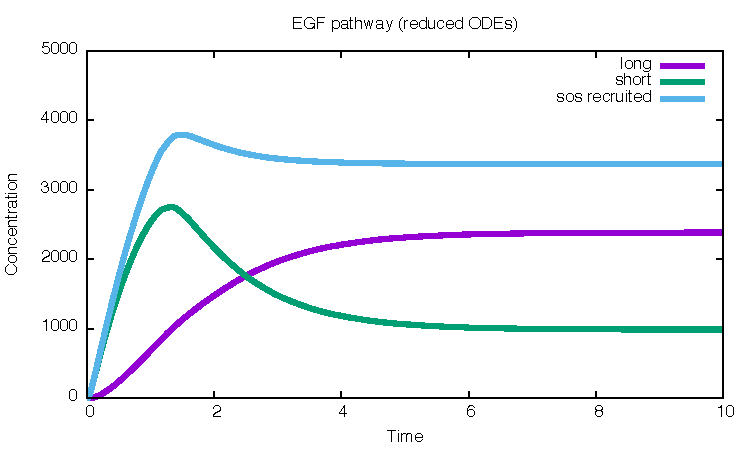
\includegraphics{generated_pictures/sos_ode_fragments.pdf}}

\hspace*{2cm}{\blue{\lang{projection exacte}{exact projection}}}

\hspace*{0.6cm}{\blue{\lang{de la sémantique différentielle}{\hspace*{5mm}of the ODE semantics}}}
\end{minipage}
\end{slide}


{\superplan}


\begin{slide}{\frametitle{A chemical species}}
\begin{minipage}{\linewidth}
\begin{center}\scalebox{0.9}{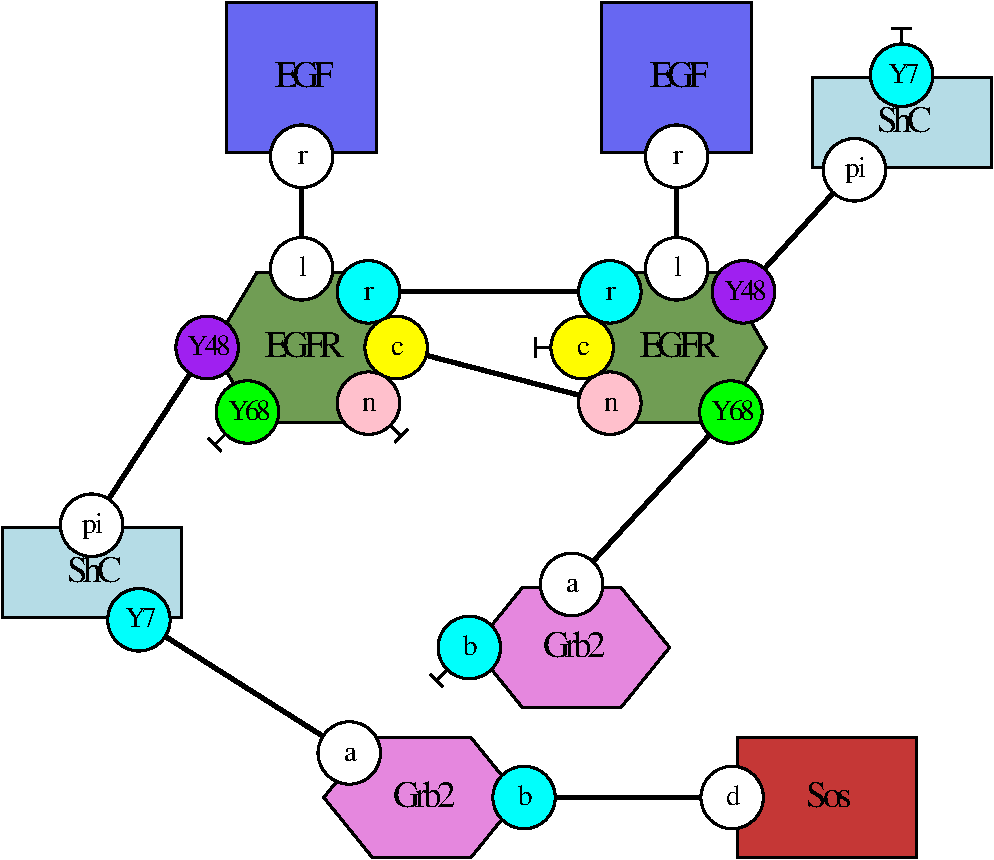
\includegraphics{generated_pictures/species.pdf}}
\end{center}
\vfill
\end{minipage}
\end{slide}

\begin{slide}{\frametitle{Receptor activation}}
\begin{minipage}{\linewidth}
\begin{center}
\scalebox{1.2}{\includegraphics{generated_pictures/rule1.pdf}}
\end{center}
\end{minipage}
\end{slide}

\begin{slide}{\frametitle{Asymmetric dimerisation}}
\begin{minipage}{\linewidth}
\begin{center}
\scalebox{1.2}{\includegraphics{generated_pictures/rule11.pdf}}
\end{center}
\vspace*{1cm}
\begin{center}
\scalebox{1.2}{\includegraphics{generated_pictures/rule12.pdf}}
\end{center}
\end{minipage}
\end{slide}


\begin{slide}{\frametitle{Sequential unbinding}}
\begin{minipage}{\linewidth}
\begin{center}
\scalebox{1.2}{\includegraphics{generated_pictures/ruled11.pdf}}
\end{center}
\vspace*{1cm}
\begin{center}
\scalebox{1.2}{\includegraphics{generated_pictures/ruled12.pdf}}
\end{center}
\end{minipage}
\end{slide}


\begin{slide}{\frametitle{Internal state}}
\begin{minipage}{\linewidth}
\begin{center}
\scalebox{1.2}{\includegraphics{generated_pictures/rule2.pdf}}
\end{center}
\end{minipage}
\end{slide}

\short{
\begin{slide}{\frametitle{Don't care, Don't write}}
\begin{minipage}{\linewidth}
\begin{center}
\scalebox{1.2}{\includegraphics{generated_pictures/rule3.pdf}}
\end{center}
\end{minipage}

\vspace*{1cm}

\begin{equation*}
{\HUGE \neq}
\end{equation*}

\vspace*{1cm}

\begin{minipage}{\linewidth}
\begin{center}
\scalebox{1.2}{\includegraphics{generated_pictures/rule4.pdf}}
\end{center}
\end{minipage}
\end{slide}



\begin{slide}{\frametitle{Side effects}}

\vfill

\begin{minipage}{\linewidth}
\begin{center}
\scalebox{1.2}{\includegraphics{generated_pictures/rule5.pdf}}
\end{center}
\end{minipage}

\vfill


\end{slide}

\begin{slide}{\frametitle{Creation/Suppression}}
\begin{minipage}{\linewidth}
\begin{center}
\scalebox{1.2}{\includegraphics{generated_pictures/rule6.pdf}}
\end{center}
\end{minipage}

\vfill

\begin{minipage}{\linewidth}
\begin{center}
\scalebox{1.2}{\includegraphics{generated_pictures/rule7.pdf}}
\end{center}
\end{minipage}
\end{slide}}


{\superplan}

\begin{slide}{\frametitle{Contact map}}

\end{slide}

\begin{slide}{\frametitle{Conflicts}}

\end{slide}

\begin{slide}{\frametitle{Self-loops}}

\end{slide}

\begin{slide}{\frametitle{Several self-loops}}

\end{slide}

\begin{slide}{\frametitle{Invariants}}

\end{slide}

\begin{slide}{\frametitle{Combinatorial complexity}}

\end{slide}

{\superplan}

\begin{slide}{\frametitle{Repeatable pattern}}

\end{slide}

\begin{slide}{\frametitle{Transitions between sites}}

\end{slide}

\begin{slide}{\frametitle{The graph of the sites}}

\end{slide}

\begin{slide}{\frametitle{Detection of unbounded polymers}}

\end{slide}

{\superplan}

\begin{slide}{\frametitle{Repeatable pattern}}

\end{slide}

\begin{slide}{\frametitle{Transitions between the edges}}

\end{slide}

\begin{slide}{\frametitle{The graph of the links}}

\end{slide}

\begin{slide}{\frametitle{Detection of unbounded polymers}}

\end{slide}

{\superplan}

\begin{slide}{\frametitle{Issues}}

\end{slide}

\begin{slide}{\frametitle{The graph of the links}}

\end{slide}

\begin{slide}{\frametitle{Labelled transitions}}

\end{slide}

\begin{slide}{\frametitle{Refinement}}

\end{slide}

{\superplan}

\end{document}
